\section{Durchführung}
\label{sec:Durchführung}
In diesem Versuch wird ein Aufbau verwendet, wie in \autoref{fig:Aufbau} zu sehen ist.
\begin{figure}[H]
    \centering
    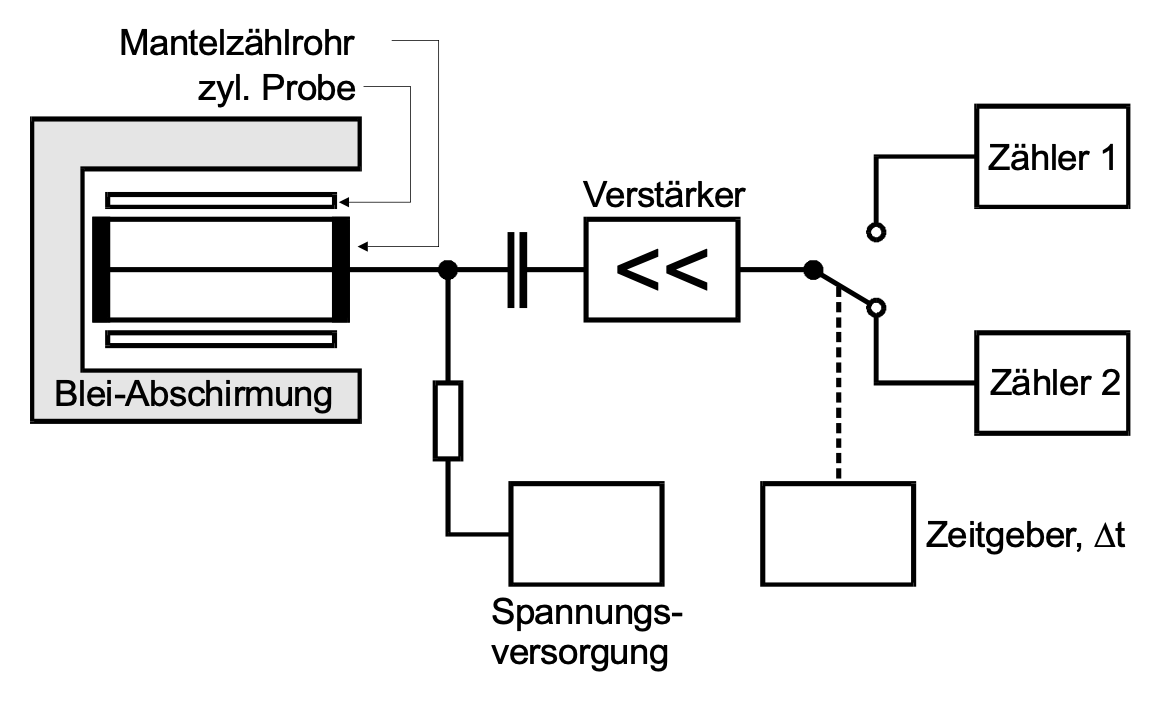
\includegraphics[height=5.5cm]{content/pics/Aufbau.png}
    \caption{Skizze des Aufbaus \cite{v702}.}
    \label{fig:Aufbau}
\end{figure}

In einem ersten Schritt wird eine Nullmessung durchgeführt. Dies bedeutet, dass kein Präparat über das Mantelzählrohr 
gestülpt wird, sondern dass lediglich die Hintergrundstrahlung über einen Zeitraum von $t=\qty{600}{\second}$ gemessen wird.
Mithilfe dieser Messung lassen sich die weiteren Messreihen um die Hintergrundstrahlung bereinigen.

Der in Abschnitt \ref{sec:Neutronenaktivierung} beschriebenen Apperatur zur Aktivierung durch Neutronen wird das aktivierte Vanadium-51
entnommen und zügig in die Messapparatur eingeführt. In einer Gesamtmesszeit von $t=\qty{900}{\second}$ werden alle $\symup{\Delta}t=\qty{30}{\second}$
die in diesem Zeitraum detektierten Zerfälle notiert.

Für Rhodium-134 wird eine Gesamtmesszeit von $t=\qty{720}{\second}$ und $\symup{\Delta}t=\qty{15}{\second}$ gewählt.